\documentclass[aspectratio=169]{beamer}

\mode<presentation>

\usepackage[utf8]{inputenc}
\usepackage[T1]{fontenc}	%makes å,ä,ö etc. proper symbols
\usepackage{amsmath}
\usepackage{graphicx}
\usepackage{xcolor}
\usepackage{listings}
\usepackage{multicol}
\usepackage{hyperref}
\usepackage[swedish]{babel}

\definecolor{LundaGroen}{RGB}{00,68,71}
\definecolor{StabilaLila}{RGB}{85,19,78}
\definecolor{VarmOrange}{RGB}{237,104,63}

\definecolor{MagnoliaRosa}{RGB}{251,214,209}
\definecolor{LundaHimmel}{RGB}{204,225,225}
\definecolor{LundaLjus}{RGB}{255,242,191}

\usefonttheme{serif}
\usetheme{malmoe}
\setbeamercolor{palette primary}{bg=LundaHimmel, fg=StabilaLila}
\setbeamercolor{palette quaternary}{bg=LundaGroen, fg=MagnoliaRosa}
\setbeamercolor{background canvas}{bg=LundaLjus}
\setbeamercolor{structure}{fg=LundaGroen}

\usepackage[many]{tcolorbox}

\newtcolorbox{cross}{blank,breakable,parbox=false,
  overlay={\draw[red,line width=5pt] (interior.south west)--(interior.north east);
    \draw[red,line width=5pt] (interior.north west)--(interior.south east);}}
    
\newcommand{\code}[1]{\colorbox{white}{\lstinline{#1}}}



\lstset{language=Python} 
\lstset{%language=[LaTeX]Tex,%C++,
    morekeywords={PassOptionsToPackage,selectlanguage,True,False},
    keywordstyle=\color{blue},%\bfseries,
    basicstyle=\small\ttfamily,
    %identifierstyle=\color{NavyBlue},
    commentstyle=\color{red}\ttfamily,
    stringstyle=\color{VarmOrange},
    numbers=left,%
    numberstyle=\scriptsize,%\tiny
    stepnumber=1,
    numbersep=8pt,
    showstringspaces=false,
    breaklines=true,
    %frameround=ftff,
    frame=single,
    belowcaptionskip=.75\baselineskip,
	tabsize=4,
	backgroundcolor=\color{white}
    %frame=L
}


\begin{document}

\lstset{literate=
  {á}{{\'a}}1 {é}{{\'e}}1 {í}{{\'i}}1 {ó}{{\'o}}1 {ú}{{\'u}}1
  {Á}{{\'A}}1 {É}{{\'E}}1 {Í}{{\'I}}1 {Ó}{{\'O}}1 {Ú}{{\'U}}1
  {à}{{\`a}}1 {è}{{\`e}}1 {ì}{{\`i}}1 {ò}{{\`o}}1 {ù}{{\`u}}1
  {À}{{\`A}}1 {È}{{\'E}}1 {Ì}{{\`I}}1 {Ò}{{\`O}}1 {Ù}{{\`U}}1
  {ä}{{\"a}}1 {ë}{{\"e}}1 {ï}{{\"i}}1 {ö}{{\"o}}1 {ü}{{\"u}}1
  {Ä}{{\"A}}1 {Ë}{{\"E}}1 {Ï}{{\"I}}1 {Ö}{{\"O}}1 {Ü}{{\"U}}1
  {â}{{\^a}}1 {ê}{{\^e}}1 {î}{{\^i}}1 {ô}{{\^o}}1 {û}{{\^u}}1
  {Â}{{\^A}}1 {Ê}{{\^E}}1 {Î}{{\^I}}1 {Ô}{{\^O}}1 {Û}{{\^U}}1
  {œ}{{\oe}}1 {Œ}{{\OE}}1 {æ}{{\ae}}1 {Æ}{{\AE}}1 {ß}{{\ss}}1
  {ű}{{\H{u}}}1 {Ű}{{\H{U}}}1 {ő}{{\H{o}}}1 {Ő}{{\H{O}}}1
  {ç}{{\c c}}1 {Ç}{{\c C}}1 {ø}{{\o}}1 {å}{{\r a}}1 {Å}{{\r A}}1
  {€}{{\euro}}1 {£}{{\pounds}}1 {«}{{\guillemotleft}}1
  {»}{{\guillemotright}}1 {ñ}{{\~n}}1 {Ñ}{{\~N}}1 {¿}{{?`}}1
}

\AtBeginSection[ ]
{
\begin{frame}{Innehåll}
    	\tableofcontents[currentsection]
\end{frame}
}

\title{Grafer i Python}
\date{vt 24}
\author{Programmering}

\maketitle

\section{Grafer}

\subsection{En graf}

\begin{frame}
\frametitle{Grafer}

\begin{figure}
\centering
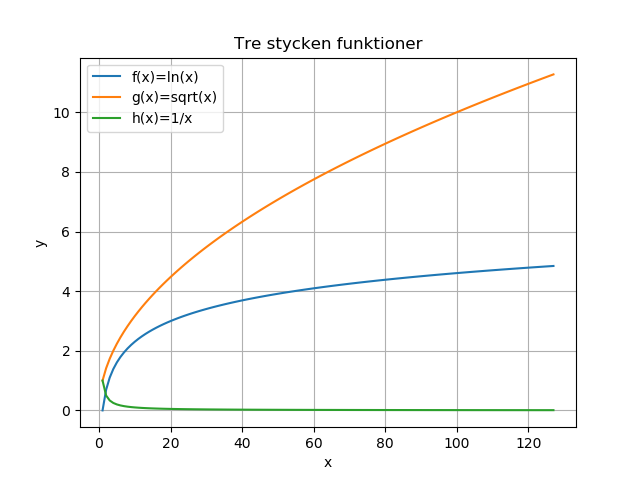
\includegraphics[width=0.5\textwidth]{Figure_1.png}
\caption{En graf gjord i Python}
\end{figure}

\end{frame}

\subsection{Vetenskap och Python}

\begin{frame}
\frametitle{Grafer}

Python anses av många vara ett programmeringsspråk väl anpasssat för beräkningar och vetenskap. En stor del av detta är tack vare biblioteken \textit{scipy, numpy} och \textit{matplotlib}.

\begin{itemize}
	\item \textit{scipy} innehåller kod för att göra numeriska analyser\\
	\item \textit{numpy} innehåller huvudsakligen datatypen \texttt{array}\\
	\item \textit{matplotlib} innehåller verktyg för grafer
\end{itemize}

\end{frame}

\section{Matplotlib}

\subsection{Installera}

\begin{frame}[fragile]
\frametitle{Matplotlib}
\framesubtitle{Installera}

För att använda \textit{matplotlib} behöver man först installera det med hjälp av \texttt{pip}.

\begin{lstlisting}
pip install matplotlib
\end{lstlisting}

Detta kommandot körs i kommandotolken på windows.

\begin{figure}
	
\includegraphics[width=0.45\textwidth]{cmd.PNG}
	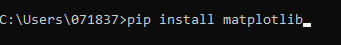
\includegraphics[width=0.45\textwidth]{cmd2.PNG}
	\caption{Skärmdump av hur man installera matplotlib}
\end{figure}

Jag föredrar dock att använda kommandot \code{python -m pip install matplotlib} enligt någon på internet så är det stabilare.

\end{frame}

\subsection{Importera}

\begin{frame}[fragile]
\frametitle{Matplotlib}
\framesubtitle{Importera till Python}

För att kunna använda biblioteket sen behöver vi i vårt program importera \textit{matplotlib}

\begin{lstlisting}
import matplotlib
\end{lstlisting}

Särskilt vill vi importera \textit{pyplot} ur \textit{matplotlib}

\begin{lstlisting}
import matplotlib.pyplot
\end{lstlisting}

Det är också vanligt att att förenkla det

\begin{lstlisting}
import matplotlib.pyploy as plt
\end{lstlisting}

\end{frame}

\section{Pyplot}

\subsection{Grundläggande användning}

\begin{frame}[fragile]
\frametitle{Pyplot}

För att sen plotta en graf skriver man följande:

\begin{lstlisting}
# Först skapar vi listor med x- och y-värden
x = [0,1,2,3,4,5,6,7,8,9,10]
y = [0,1,4,9,16,25,36,49,64,81,100]
# Sen placerar vi ut dem i grafen
plt.plot(x,y)
# Sist så visar vi grafen
plt.show()
\end{lstlisting}

\begin{figure}
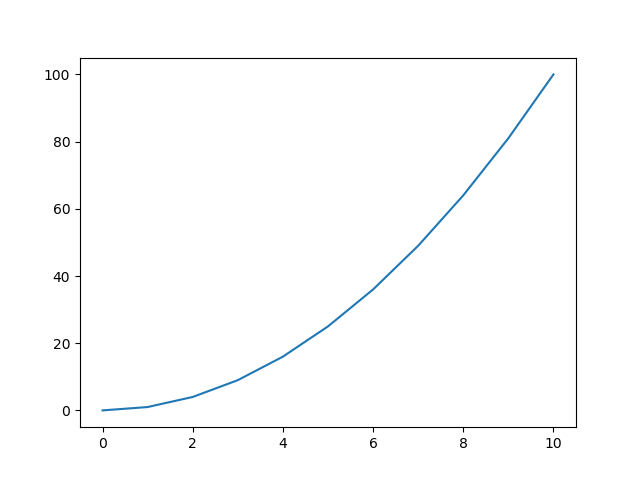
\includegraphics[width = 0.2\textwidth]{squares.png}
\caption{$y=x^2$}
\end{figure}

\end{frame}

\subsection{Axlarna}

\begin{frame}[fragile]
\frametitle{Pyplot}
\framesubtitle{Axel-rubriker}

\centering
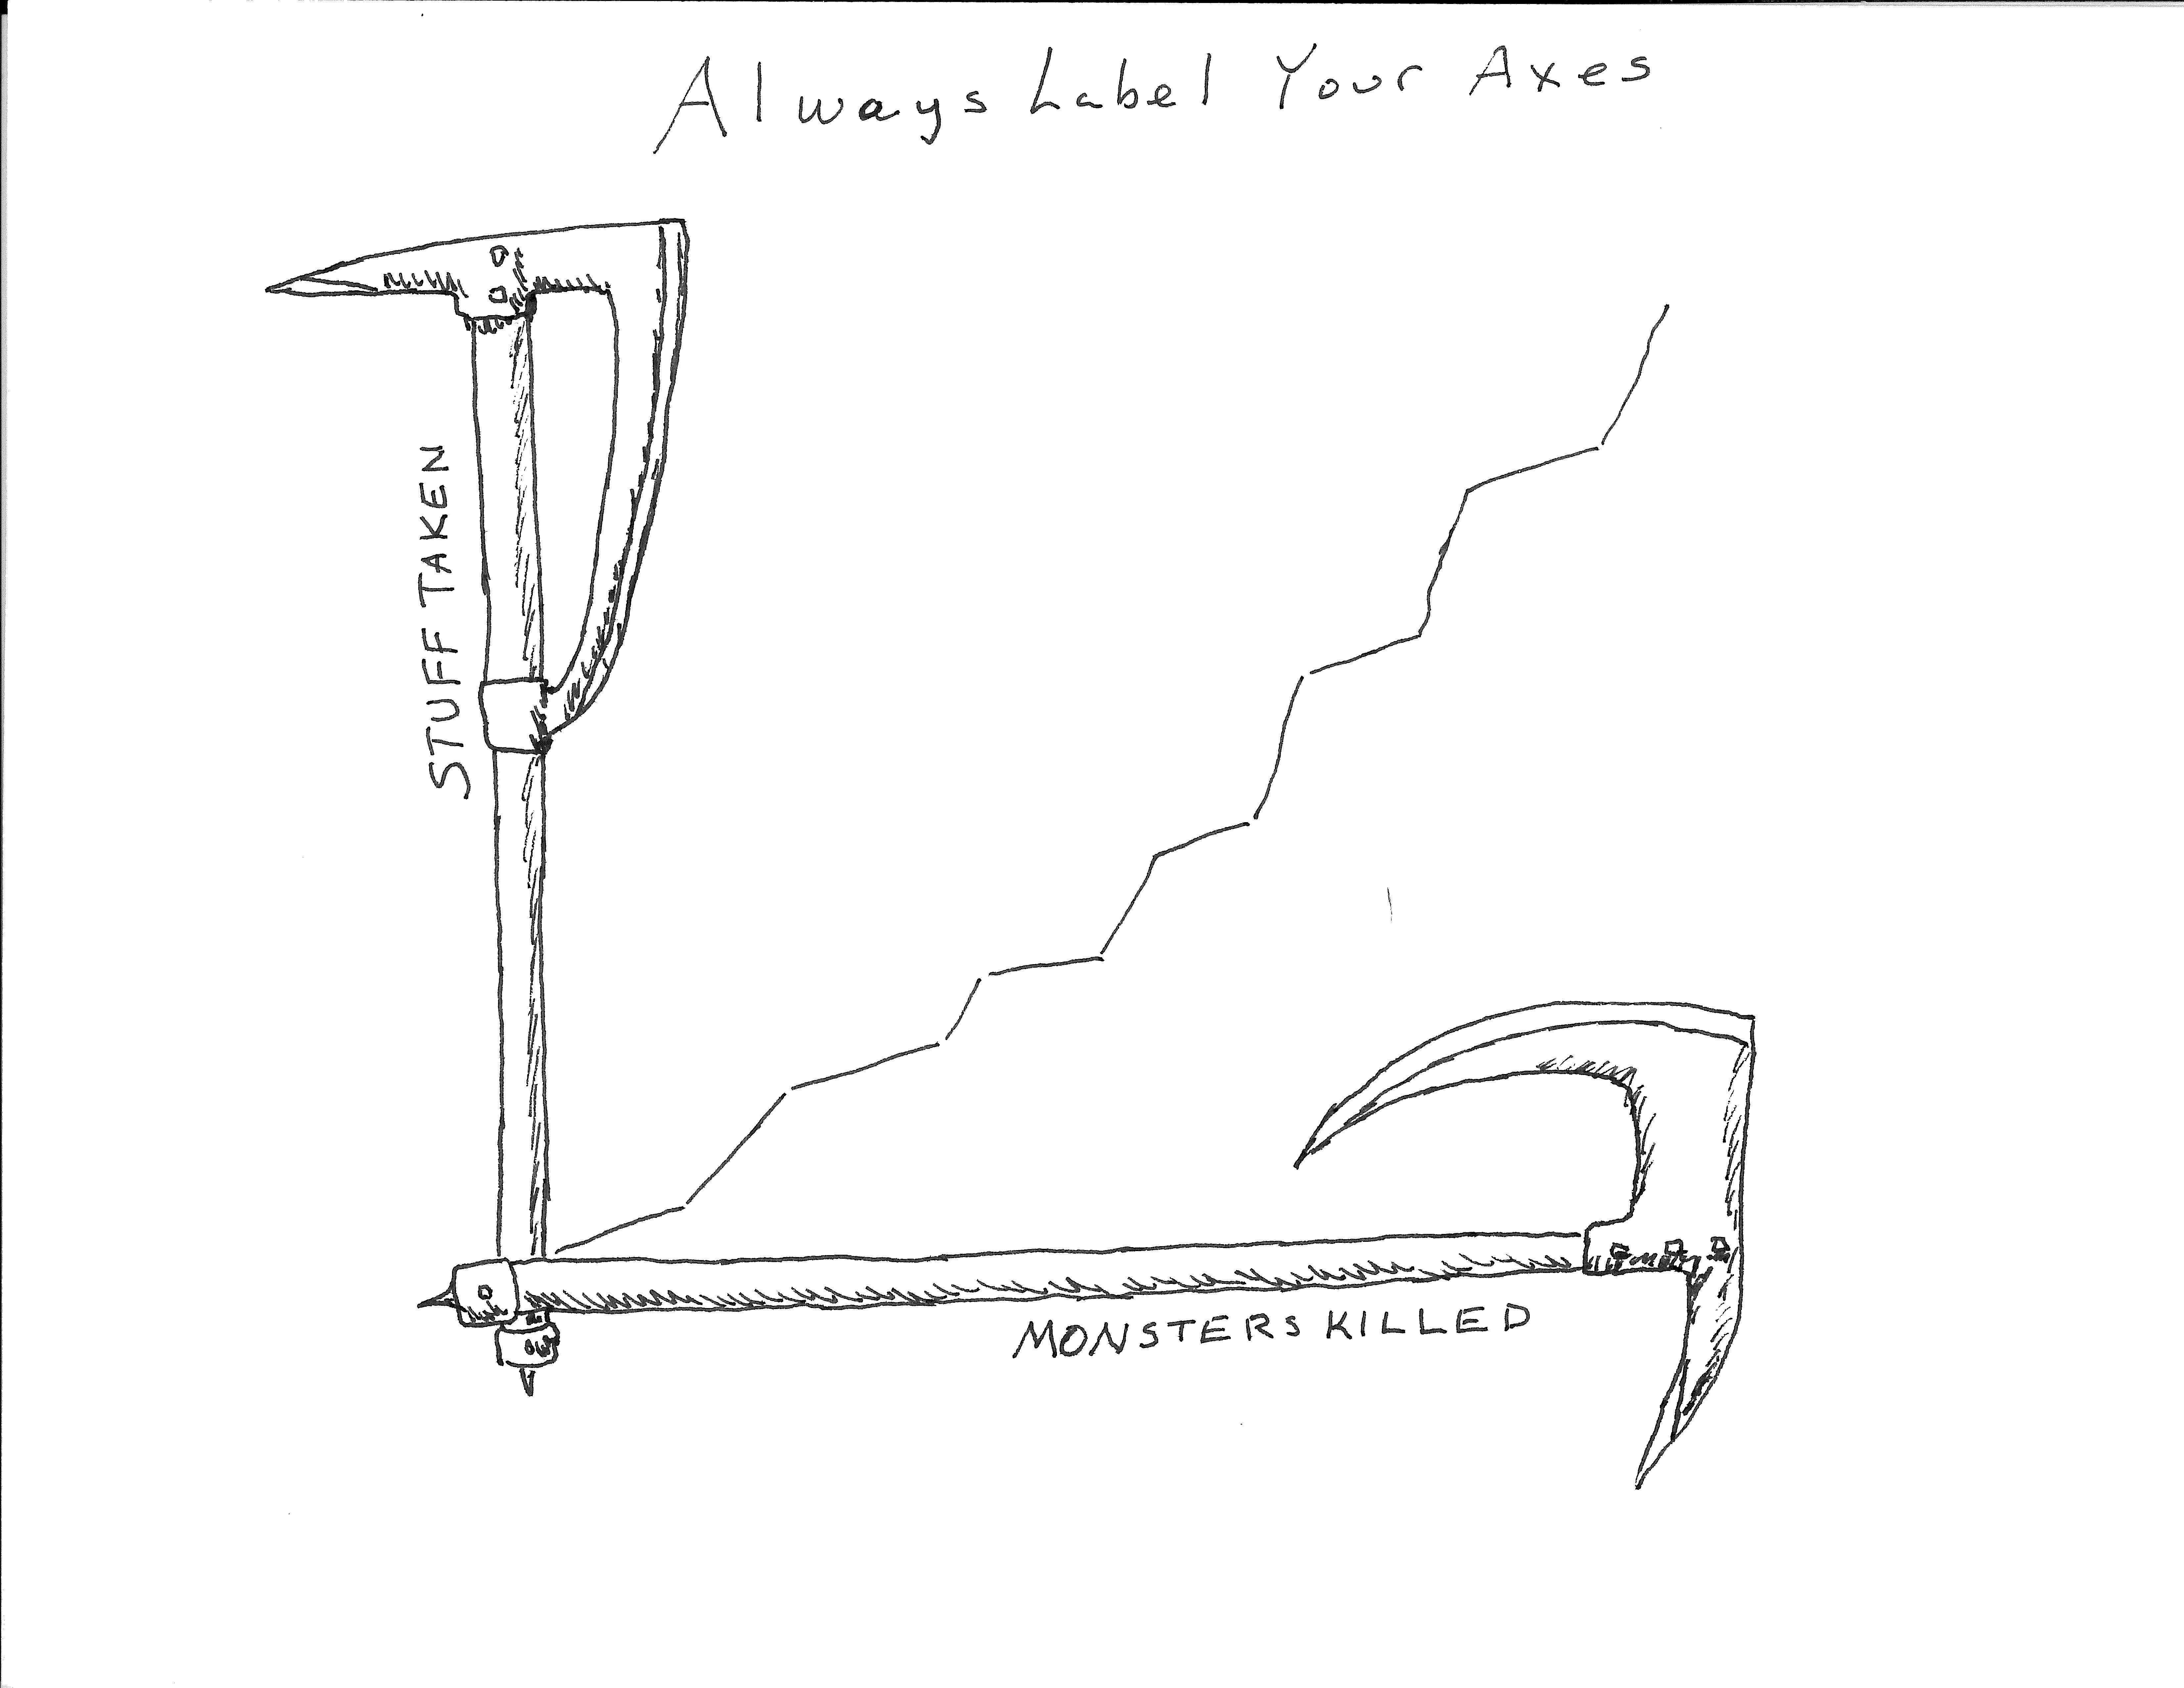
\includegraphics[width=.5\textwidth]{labelyouraxes.jpg}

\end{frame}

\begin{frame}[fragile]
\frametitle{Pyplot}
\framesubtitle{Axel-rubriker}

\begin{lstlisting}
import matplotlib.pyplot as plt
x = [0,1,2,3,4,5,6,7,8,9,10]
y = [0,1,4,9,16,25,36,49,64,81,100]
plt.plot(x,y)
plt.xlabel('x') # Sätter en titel på x-axeln
plt.ylabel('y') # Sätter en titel på y-axeln
plt.show()
\end{lstlisting}

\end{frame}

\begin{frame}
\frametitle{Pyplot}

\begin{figure}
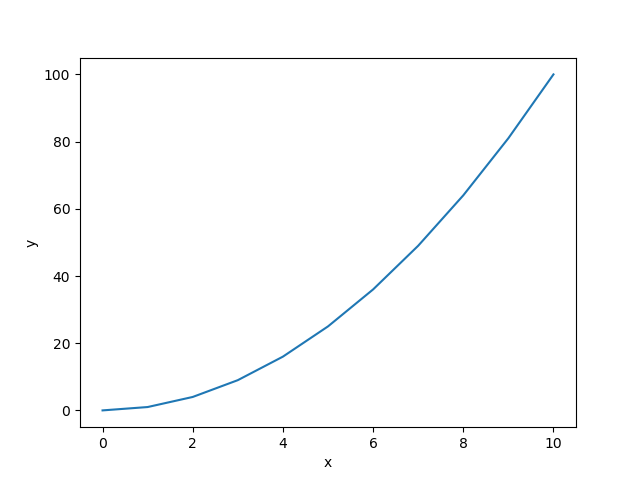
\includegraphics[width = 0.5\textwidth]{squares2.png}
\caption{$y=x^2$}
\end{figure}

\end{frame}

\subsection{Rubrik}

\begin{frame}[fragile]
\frametitle{Pyplot}
\frametitle{Rubriker}

\begin{lstlisting}
import matplotlib.pyplot as plt
x = [0,1,2,3,4,5,6,7,8,9,10]
y = [0,1,4,9,16,25,36,49,64,81,100]
plt.plot(x,y)
plt.xlabel('x')
plt.ylabel('y')
plt.title('f(x)=x^2') # Lägger till en rubrik
plt.show()
\end{lstlisting}

\end{frame}

\begin{frame}
\frametitle{Rubrik}

\begin{figure}
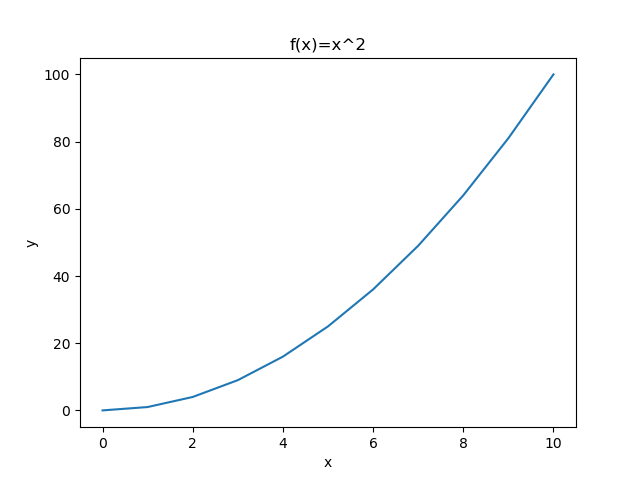
\includegraphics[width = 0.5\textwidth]{squares3.png}
\caption{En graf med allt!}
\end{figure}

\end{frame}

\begin{frame}
\frametitle{Pyplot}
\framesubtitle{Kommandon}

\begin{tabular}{| l | p{7cm}|}
\hline
\textbf{Kommando}	& \textbf{Effekt}\\ \hline
\code{plt.plot(x,y)}	& Plottar $x$ som en funktion av $y$\\
\code{plt.show()}	& Visar grafen.\\
\code{plt.xlabel('text')} & Ger x-axeln rubrik\\
\code{plt.ylabel('text')} & Ger y-axeln rubrik\\
\code{plt.title('text')}	& Ger grafen en titel\\
\code{plt.grid()}		& Lägger till ett rutnät\\ \hline
\end{tabular}\\

Fler kommandon kan man hitta \color{blue}{\href{https://matplotlib.org/3.1.1/api/pyplot_summary.html}{här}}.

\end{frame}

\begin{frame}
\frametitle{Fler grafer}

\href{https://www.machinelearningplus.com/plots/top-50-matplotlib-visualizations-the-master-plots-python/}{Top 50 matplotlib visualizations: The Master Plots}

\end{frame}

\section{Funktioner}

\begin{frame}[fragile]
\frametitle{Funktioner}
\framesubtitle{Skitsnabbt}

\begin{lstlisting}
def f(x):
    # Skriv kod här
    y = x**2+3*x-1/x
    return y
\end{lstlisting}

\end{frame}

\begin{frame}[fragile]
	\frametitle{Funktioner och plottar}

	\begin{itemize}
		\item Ett sätt att använda funktioner med sina plottar är:
	\end{itemize}
	
	\begin{lstlisting}
import matplotlib.pyplot as plt

def f(x):
    return x**2
    
x_data = [x for x in range(0,10)]
y_data = [f(x) for x in x_data] 
plt.plot(x,y)
plt.show()
	\end{lstlisting}

\end{frame}

\section{Övningar}

\begin{frame}
\frametitle{Övningar}

	\begin{itemize}
		\item Rita ut grafen för funktionen \(f(x)=1.5^x, -5\leq x\leq5\)
		\item Rita ut grafen för funktionen \(g(x)=x^2+3x-\dfrac{1}{x}, -5\leq x\leq5\)
		\item Få grafen att inte dra streck mellan punkterna
		\item Rita ut alla grafer i samma diagram.
	\end{itemize}

\end{frame}

\end{document}